\documentclass{article}
\usepackage[a4paper]{geometry}
\usepackage[skip=10pt]{parskip}
\usepackage{graphicx}
\usepackage{hyperref}
\usepackage[section]{placeins}
\usepackage[official]{eurosym}
\usepackage{textgreek}
\usepackage{tcolorbox}
\usepackage{listings}
\usepackage{textcomp}
\usepackage{multirow}
\usepackage{tikz}

\setlength\parindent{0pt}

\newenvironment{note}{\begin{tcolorbox}[colback=blue!5!white,colframe=blue!75!black,title=\textbf{Note}]}{\end{tcolorbox}}
\newenvironment{caution}{\begin{tcolorbox}[colback=red!5!white,colframe=red!75!black,title=\textbf{Caution}]}{\end{tcolorbox}}
\newcommand{\datasheet}{\href{https://ww1.microchip.com/downloads/en/DeviceDoc/doc2593.pdf}{datasheet}}
\newcommand{\file}[1]{\texttt{#1}}
\newcommand{\evaboard}{\href{https://github.com/7vgn/EvaBoard/}{evaluation board}}

\lstset
{
	basicstyle=\footnotesize\ttfamily,
	breaklines=true,
	keywordstyle=\bfseries\color{green!40!black},
	commentstyle=\itshape\color{purple!40!black},
	identifierstyle=\color{blue},
	stringstyle=\color{orange},
	tabsize=4
}

\begin{document}
\hypersetup{pageanchor=false}
\begin{titlepage}
\thispagestyle{empty}
\centering
\textsf{\Huge Guide Book}\\[1cm]
\textsf{\Large For the AD/DA Add-On Board}\\[3cm]
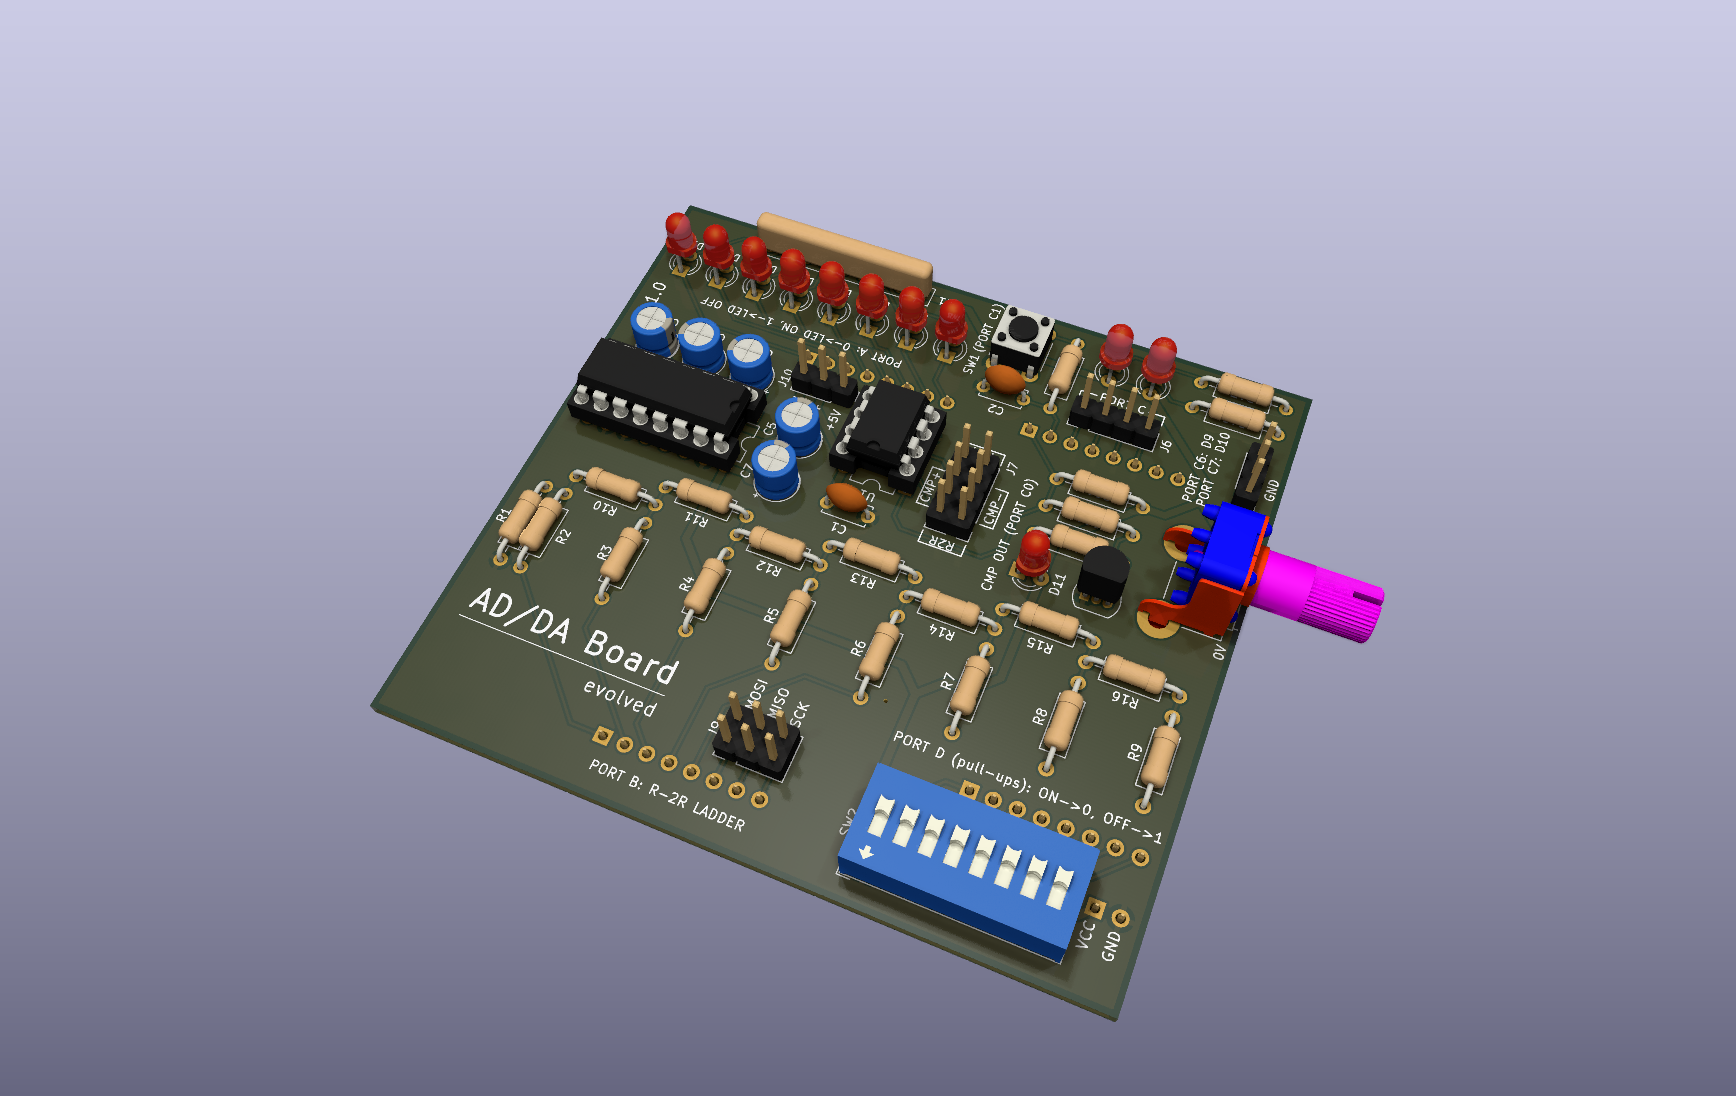
\includegraphics[width=\textwidth]{Pictures/ADDABoard3DRender.png}
\end{titlepage}
\hypersetup{pageanchor=true}

\tableofcontents
\section{Introduction}
This is an add-on for the ATmega644(A) \evaboard. It is inspired by (and compatible with) the \href{https://www.embedded.rwth-aachen.de/doku.php?id=lehre:atmegaevaboard}{add-on board} used in the lab course "Praktikum Systemprogrammierung" in the computer science curriculum at RWTH Aachen. 

The university encourages students and educators to build the evaluation board themselves. However, no resources for the AD/DA add-on board are provided. 

This project is a complete remake of the original add-on board with a focus on low cost and a non-lab environment (no bench supply etc.). It also includes a ton of documentation, especially for students who have not worked with electronics before. 

\begin{note}
Before reading this, you should familiarize yourself with the \evaboard. Many things from its documentation apply here as well and this document can only be considered complete in conjunction with the \href{../../EvaBoard/Guide/EvaBoardGuide.pdf}{evaluation board's Guide Book}.
\end{note}

\subsection{Getting to Know the Add-On Board}\label{sec:boardOverview}
This add-on board carries multiple components that can be used separately or wired together to create an AD converter:
\begin{itemize}
\item A digital-to-analogue (DA) converter in the shape of an R-2R ladder
\item A comparator with multiple power supply options
\item A potentiometer to create analogue voltages
\item 10 LEDs, a button, and an 8-bit DIP switch
\end{itemize}

For more details, refer to the \href{../KiCAD/Schematic.pdf}{schematic}. 

The add-on board plugs into connectors J11..J14 (Port A..D) and J4 (power) of the evaluation board. Table \ref{tab:connections} shows the connections between the ATmega and the add-on components when the add-on board is mounted. 
\begin{table}
\centering
\begin{tabular}{l|l|l}
\textbf{ATmega644}&\textbf{AD/DA add-on board}&\textbf{Remarks}\cr\hline
Pin A0..A7&LEDs 1..8&active low\cr\hline
Pin B0..B7&R-2R ladder&Pin B7 is the MSB\cr\hline
Pin C0&Comparator output&LED11 also shows the comparator output\cr\hline
Pin C1&Button SW1&pull-up on Pin C1 must be enabled\cr\hline
Pin C2..C5&passed through to J6&not usable while JTAG programming\cr\hline
Pin C6, C7&LEDs 9 and 10&active low\cr\hline
Pin D0..D7&8-bit DIP switch&pull-ups on Port D must be enabled\cr\hline
\end{tabular}
\caption{Connections between the Add-On Board and the Evaluation Board}
\label{tab:connections}
\end{table}

\subsubsection{R-2R Ladder}
An \href{https://en.wikipedia.org/wiki/Resistor_ladder}{R-2R ladder} is a simple circuit that converts a digital value to an analogue voltage using a network of resistors with two different values, one twice as large as the other (1k\textOmega{} and 2k\textOmega{} in our case). 
The R-2R ladder is connected to Port B in such a way that a digital value written to the 8-bit PORTB register is translated proportionally to a voltage between 0V and 5V. The output voltage is available on two pins of J7. 

\begin{note}
Pins 5..7 of Port B are also used for ISP programming. The R-2R ladder will act as a pull-down resistor on these pins. Decent ISP programmers should not have an issue with this. If you encounter difficulties, remove the add-on board while programming or cut the solder jumpers JP1..JP3. You can reconnect these pins to the R-2R ladder by placing jumpers on J9. 
\end{note}

\subsubsection{Comparator}\label{sec:cmp}
The \href{https://www.ti.com/lit/ds/symlink/lm393.pdf}{LM393} is a very common dual comparator. On this board, only one of the two comparators is in use. The comparator has two inputs \texttt{IN+} and \texttt{IN-} and one output. The output is high (logic 1) whenever the voltage at \texttt{IN+} is greater than the voltage at \texttt{IN-}, and low (logic 0) whenever the opposite is the case. The two inputs are available at the middle pins of J7. The output is connected to Port C0 as well as LED11 (``CMP OUT''). 

Figure \ref{fig:cmpSchematic} shows the schematic symbol of a comparator. It resembles that of an operational amplifier. This is not a coincidence: OpAmps can be used as comparators (with mediocre performance). 

\begin{figure}[htb]
\centering
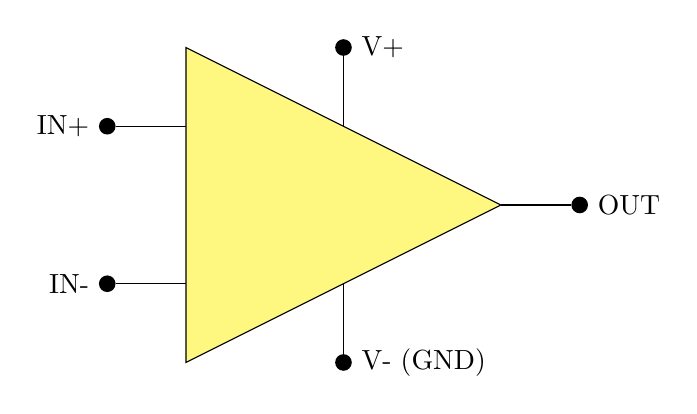
\begin{tikzpicture}
\node[circle,fill,minimum size=6pt,inner sep=0,outer sep=0,label=left:IN+] (INP) at (-1,1) {};
\node[circle,fill,minimum size=6pt,inner sep=0,outer sep=0,label=left:IN-] (INM) at (-1,-1) {};
\node[circle,fill,minimum size=6pt,inner sep=0,outer sep=0,label=right:OUT] (OUT) at (5,0) {};
\node[circle,fill,minimum size=6pt,inner sep=0,outer sep=0,label=right:V+] (VP) at (2,2) {};
\node[circle,fill,minimum size=6pt,inner sep=0,outer sep=0,label=right:V- (GND)] (VM) at (2,-2) {};

\filldraw[fill=yellow!50!white] (0,2) -- (0,-2) -- (4,0) -- cycle;
\draw (INP) -- (0,1);
\draw (INM) -- (0,-1);
\draw (4,0) -- (OUT);
\draw (VP) -- (2,1);
\draw (VM) -- (2,-1);
\end{tikzpicture}
\caption{Comparator Schematic}
\label{fig:cmpSchematic}
\end{figure}

The comparator needs a supply voltage which has to be at least 2V higher than the \texttt{IN+} and \texttt{IN-} voltages (see Section 6.2 in the \href{https://www.ti.com/lit/ds/symlink/lm393.pdf}{datasheet}). Since we want to compare voltages in the 0V..5V range, the comparator must be supplied with at least 7V which is not immediately available on the evaluation board. There are three options:

\begin{itemize}
\item Provide an external supply voltage $\ge$7V between V+ (the middle pin of J10) and GND (J8). Depending on the quality of the external supply, this can be the most stable solution and provide the most accurate results. 
\item Use 5V as the power supply by connecting the middle and bottom pin of J10 with a jumper. This limits the usable range of the comparator to 0V..3V!
\item Create a higher voltage from 5V. Fortunately, the comparator does not draw a lot of current. Thus we can (ab)use a MAX232 driver which creates a voltage somewhere between 8V and 9V, depending on current. You don't even need to buy a MAX232 -- you can pinch the one from the evaluation board, unless you want to use the serial connection and the AD/DA add-on board at the same time. Insert the MAX232 into the U2 socket of the add-on board and connect the middle and top pin of J10 with a jumper. 
\end{itemize}

The third option is recommended since it is cheap while still delivering good results. Figure \ref{fig:cmpSupplyOptions} shows the role of J10 in choosing the comparator supply voltage. 
\begin{figure}[htb]
\centering
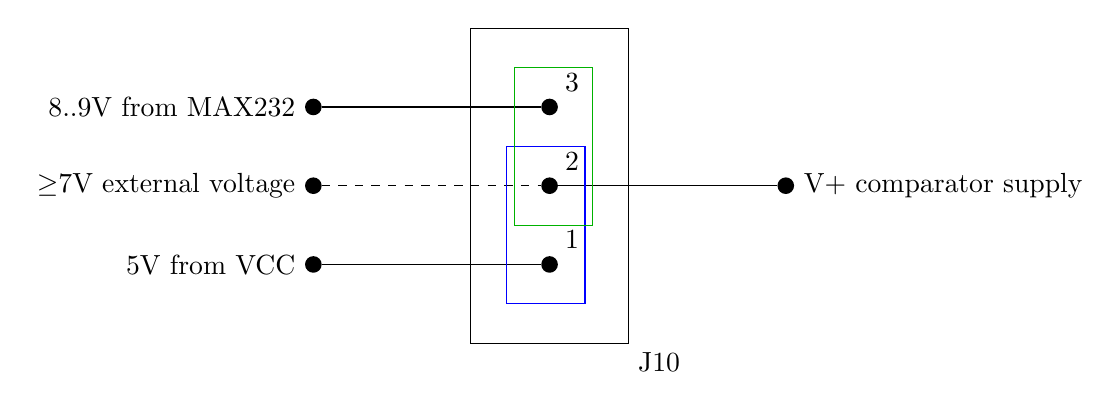
\begin{tikzpicture}
\node[circle,fill,minimum size=6pt,inner sep=0,outer sep=0,label=left:8..9V from MAX232] (MAX) at (0,3) {};
\node[circle,fill,minimum size=6pt,inner sep=0,outer sep=0,label=left:$\ge$7V external voltage] (EXT) at (0,2) {};
\node[circle,fill,minimum size=6pt,inner sep=0,outer sep=0,label=left:5V from VCC] (VCC) at (0,1) {};
\node[circle,fill,minimum size=6pt,inner sep=0,outer sep=0,label=right:V+ comparator supply] (VP) at (6,2) {};

\draw (2,0) rectangle (4,4);
\node[anchor=north west] at (4,0) {J10};
\node[circle,fill,minimum size=6pt,inner sep=0,outer sep=0,label=above right:1] (J1) at (3,1) {};
\node[circle,fill,minimum size=6pt,inner sep=0,outer sep=0,label=above right:2] (J2) at (3,2) {};
\node[circle,fill,minimum size=6pt,inner sep=0,outer sep=0,label=above right:3] (J3) at (3,3) {};

\draw (MAX) -- (J3);
\draw (VCC) -- (J1);
\draw[dashed] (EXT) -- (J2);
\draw (J2) -- (VP);

\draw[draw=blue] (2.45,0.5) rectangle (3.45,2.5);
\draw[draw=green!70!black] (2.55,1.5) rectangle (3.55,3.5);
\end{tikzpicture}
\caption{Comparator Supply Voltage Options}
\label{fig:cmpSupplyOptions}
\end{figure}

\subsubsection{Potentiometer}\label{sec:poti}
Since the whole purpose of an AD converter is to measure some analogue voltage, we need a way of generating one. The potentiometer R22 acts as a variable voltage divider between 5V and GND. When turned all the way to the left, its output is 0V, to the right it's 5V. The potentiometer output is available on two pins of J7. If you have a variable external voltage source available, you can of course omit R22. 

\subsection{Changes from the Original Board}\label{sec:differences}
No schematic is published for the original AD/DA board. Figure \ref{fig:addaOrig} is our best guess of what it looks like. 

\begin{figure}[htb]
\centering
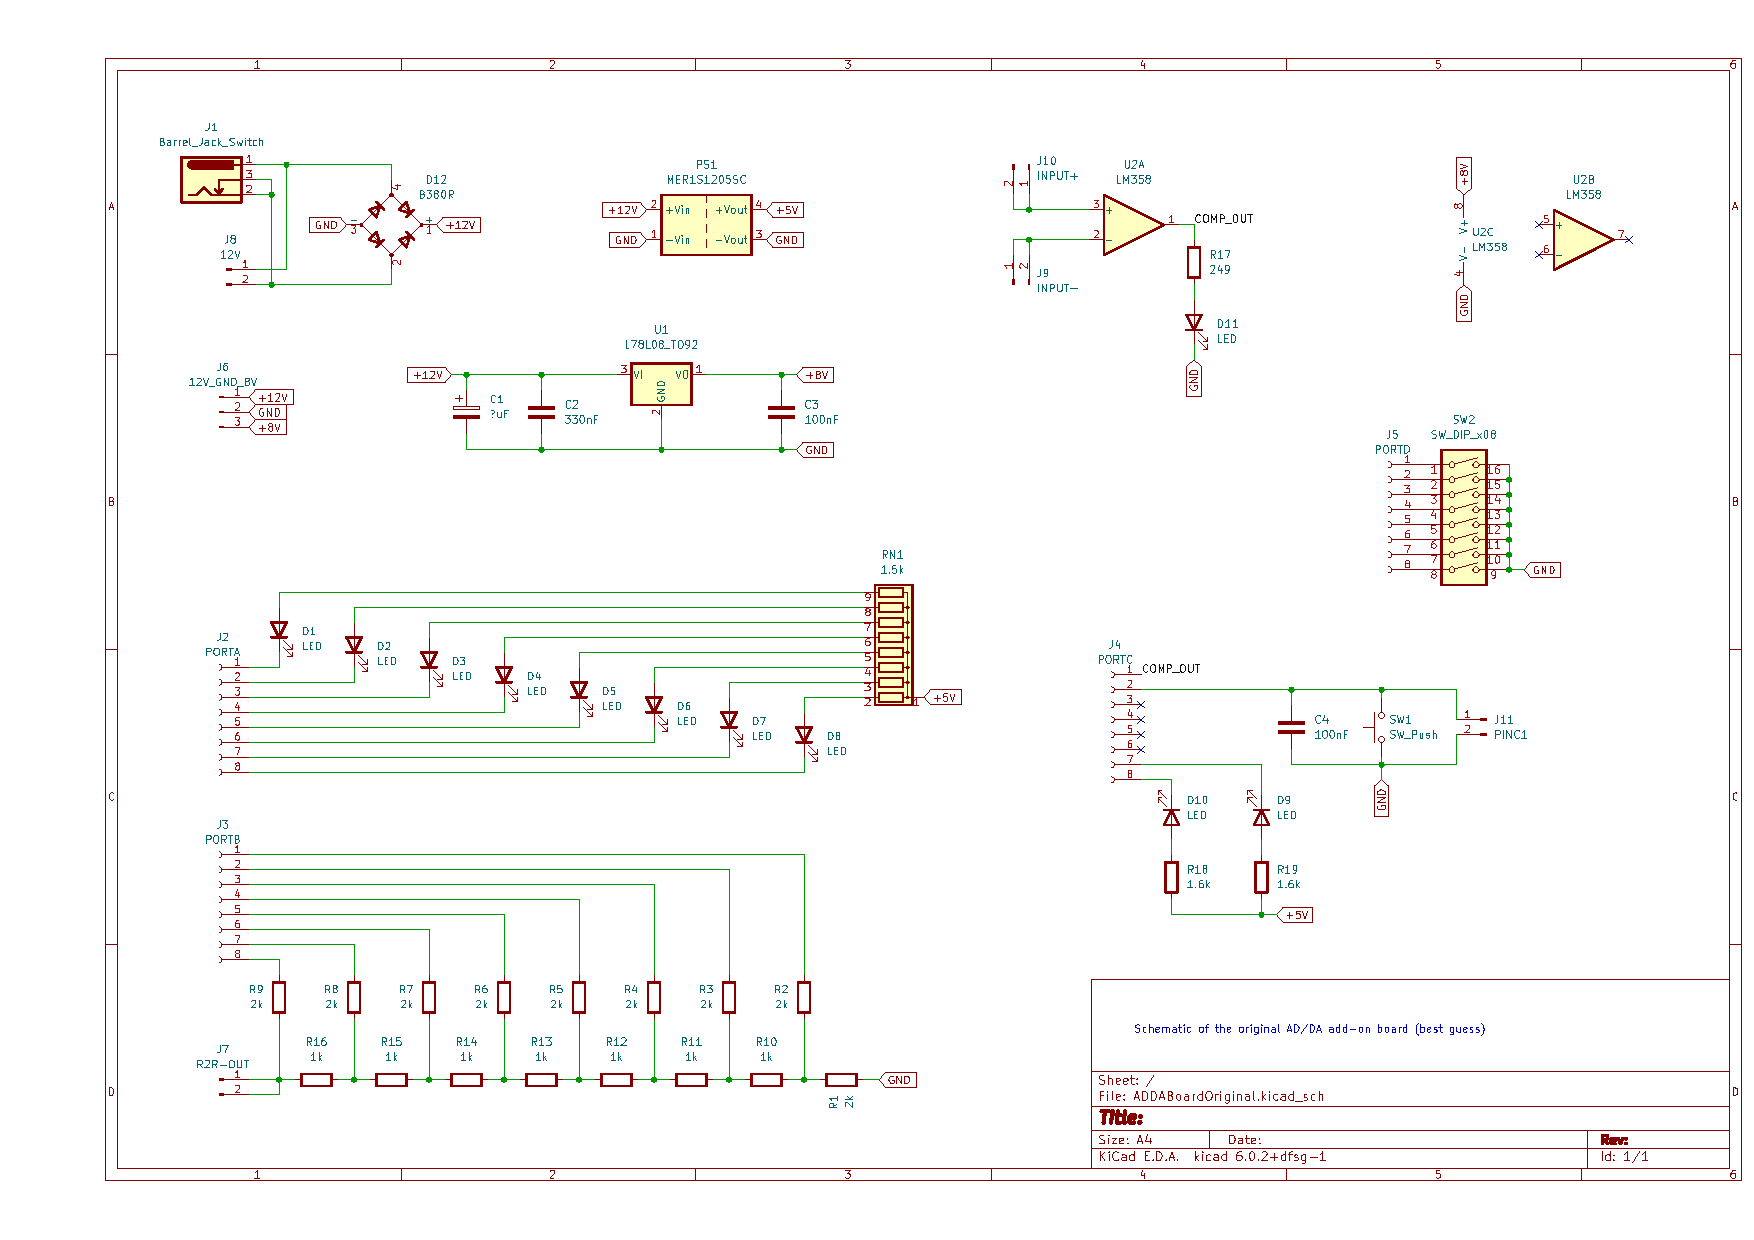
\includegraphics[width=\textwidth]{Pictures/ADDABoardOriginal.pdf}
\caption{Schematic of the Original AD/DA Add-on Board (guesswork)}
\label{fig:addaOrig}
\end{figure}

The main difference is the use of the LM393 comparator instead of an LM358 OpAmp and its power supply. Re-using the MAX232 instead of two additional voltage regulators lowers the cost of this board significantly. 

\section{Building the Board}
Please read the corresponding chapter in the evaluation board's \href{https://github.com/7vgn/EvaBoard/Guide/EvaBoardGuide.pdf}{guide book}. Assembling the add-on board should not pose any additional difficulties. 

\begin{note}
The best technique for soldering the pin sockets J1..J5 onto the back of the PCB is to attach them to the (unpowered!) evaluation board, then place the add-on PCB on top and solder all pins. This way, the add-on board will fit perfectly onto the evaluation board. 
\end{note}

\begin{caution}
Make sure to cut all the components' legs short enough so they won't touch anything on the evaluation board. To be safe, cover the back of the add-on board with tape. 
\end{caution}

\subsection{Optional Components}
The potentiometer R22 can be omitted in favour of an external variable voltage source, see Section \ref{sec:poti}. 

If the ATmega is programmed exclusively via JTAG, J6 is unnecessary since those pins aren't usable anyway. 

J9 can be left unpopulated unless you need to cut the solder jumpers JP1..3 due to problems with ISP programming while the R-2R ladder is connected to Port B. 

The IC socket for U2 as well as C3..C7 can be omitted if you are providing the comparator with a different supply voltage, see Section \ref{sec:cmp}. 

If you are using tantalum capacitors for C3..C7, make sure to get the polarity correct. Unfortunately, the markings are not uniform. The plus side might be marked by a plus sign, a line, a dot, or a longer leg. If there is text printed on it, the plus side is usually on the right. If in doubt, \href{https://en.wikipedia.org/wiki/Tantalum_capacitor#Polarity_marking}{read up} on it before soldering -- with the wrong polarity tantalum capacitors can explode!

\section{Testing}
The test programs can be found in the \href{../Tests/}{\file{Tests/} subdirectory} of this repository. They all come with makefiles for AVR-GCC and AVRDUDE. Alternatively, you can create a project in your IDE of choice and import the source files there. Be sure to define the \lstinline[language=C]{F_CPU} constant if your IDE doesn't do that automatically.

\subsection{DIP switches and LEDs}
The code for this test can be found in \href{../Tests/DIPLED/}{\file{Tests/DIPLED/}}. 

\paragraph{Preparation}
Plug the AD/DA add-on board onto the evaluation board. 

\paragraph{Expected Result}
Whenever a DIP switch is activated, the corresponding LED should light up. Pressing the SW1 should switch between LED9 and LED10. 

\begin{figure}[htb]
\centering
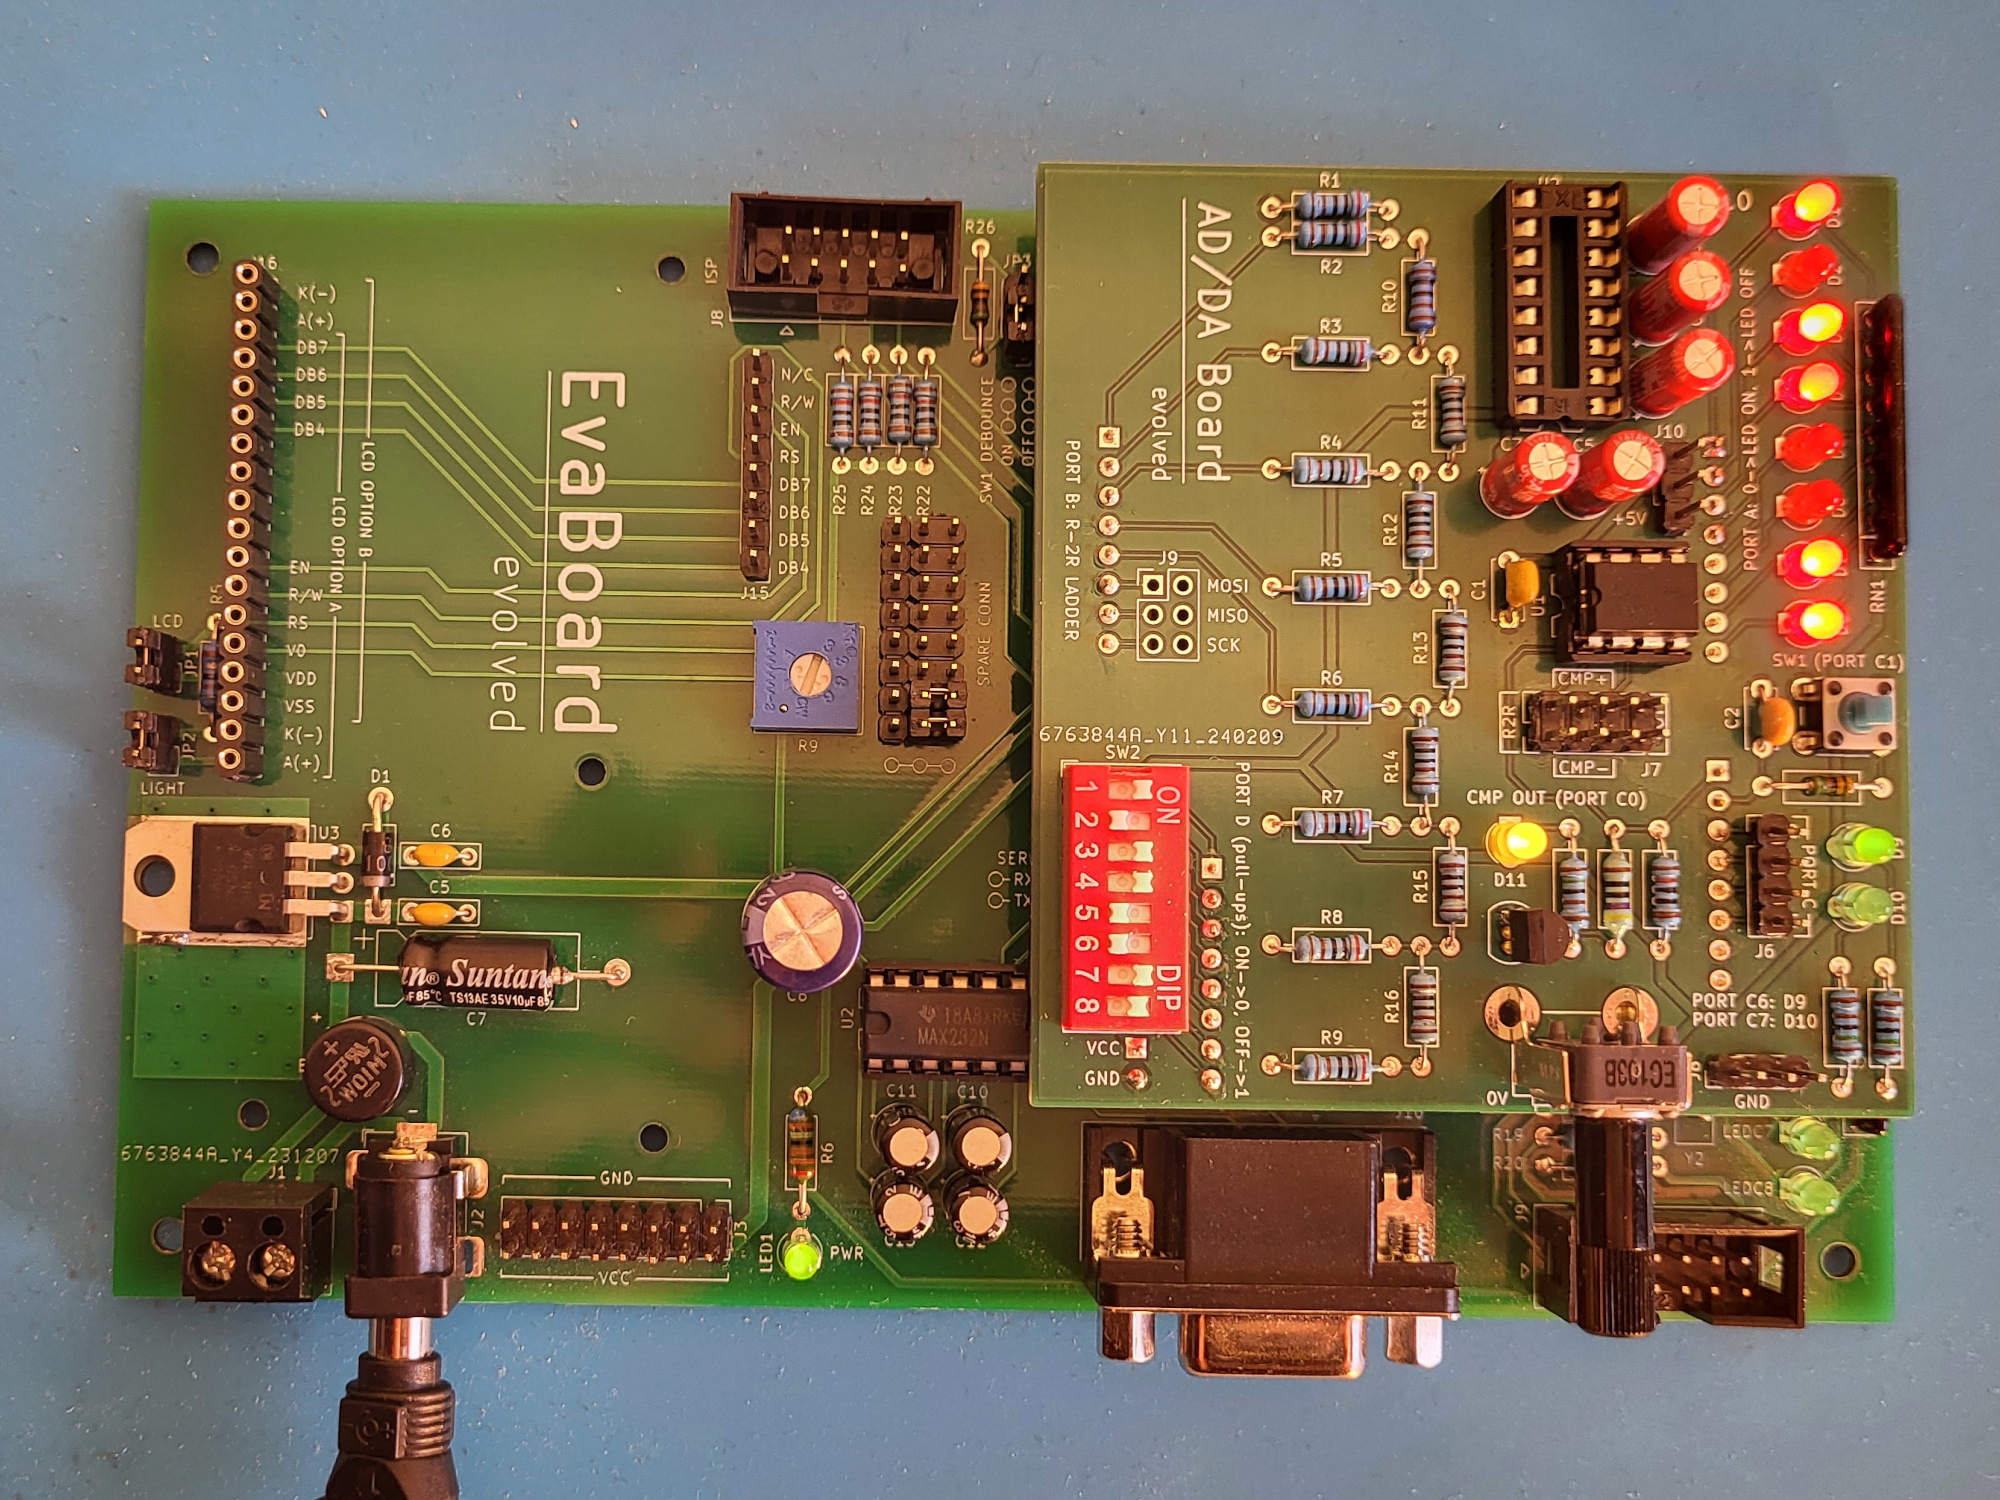
\includegraphics[width=.85\textwidth]{Pictures/DIPLED.jpg}
\caption{Setup for Testing the DIP Switches and LEDs}
\label{fig:dipLed}
\end{figure}

\paragraph{Troubleshooting}
Make sure the evaluation board works reliably. After that, any failure on this simple test is probably due to bad soldering or an LED being placed the wrong way. 

\subsection{R-2R Ladder}
The code for this test can be found in \href{../Tests/R2R/}{\file{Tests/R2R/}}. This test requires a somewhat accurate multimeter. 

\paragraph{Preparation}
Plug the AD/DA add-on board onto the evaluation board. 

\paragraph{Expected Result}
Enter a value $v\in\{0,\ldots,255\}$ in binary via the DIP switches. It should be echoed on the LEDs. Measure the voltage $U$ between the R2R pins on J7 and GND (J8). You should get approximately the following relation:
\[
U=5V\cdot\frac{v}{255}
\]
For a more precise result, measure the supply voltage (pin marked ``+5V'' on J10) and replace the ``5V'' in the equation with that value. 

\paragraph{Troubleshooting}
If the observed values deviate significantly from the expected ones, check if you have chosen the correct values for all resistors. You might also have a bad solder joint on one of the resistors, adding a few ohms. 

\begin{note}
When one of the ATmega's output pins is set to logic 1, its voltage does not quite reach VCC\footnote{The \href{https://ww1.microchip.com/downloads/en/DeviceDoc/doc2593.pdf}{datasheet} guarantees 4.2V, see Section 26.2. The exact value depends on the current sourced from the pin, see Figure 27-31.}. Therefore, the observed values will probably all have a slight downward bias. 
\end{note}

\subsection{A Primitive AD converter}
The code for this test can be found in \href{../Tests/ADC/}{\file{Tests/ADC/}}. 

\paragraph{Preparation}
Plug the AD/DA add-on board onto the evaluation board. Connect R-2R to CMP+ and POT to CMP- by placing two jumpers on J7. 
Use one of the methods from Section \ref{sec:cmp} to supply the comparator with voltage. 

\begin{figure}[htb]
\centering
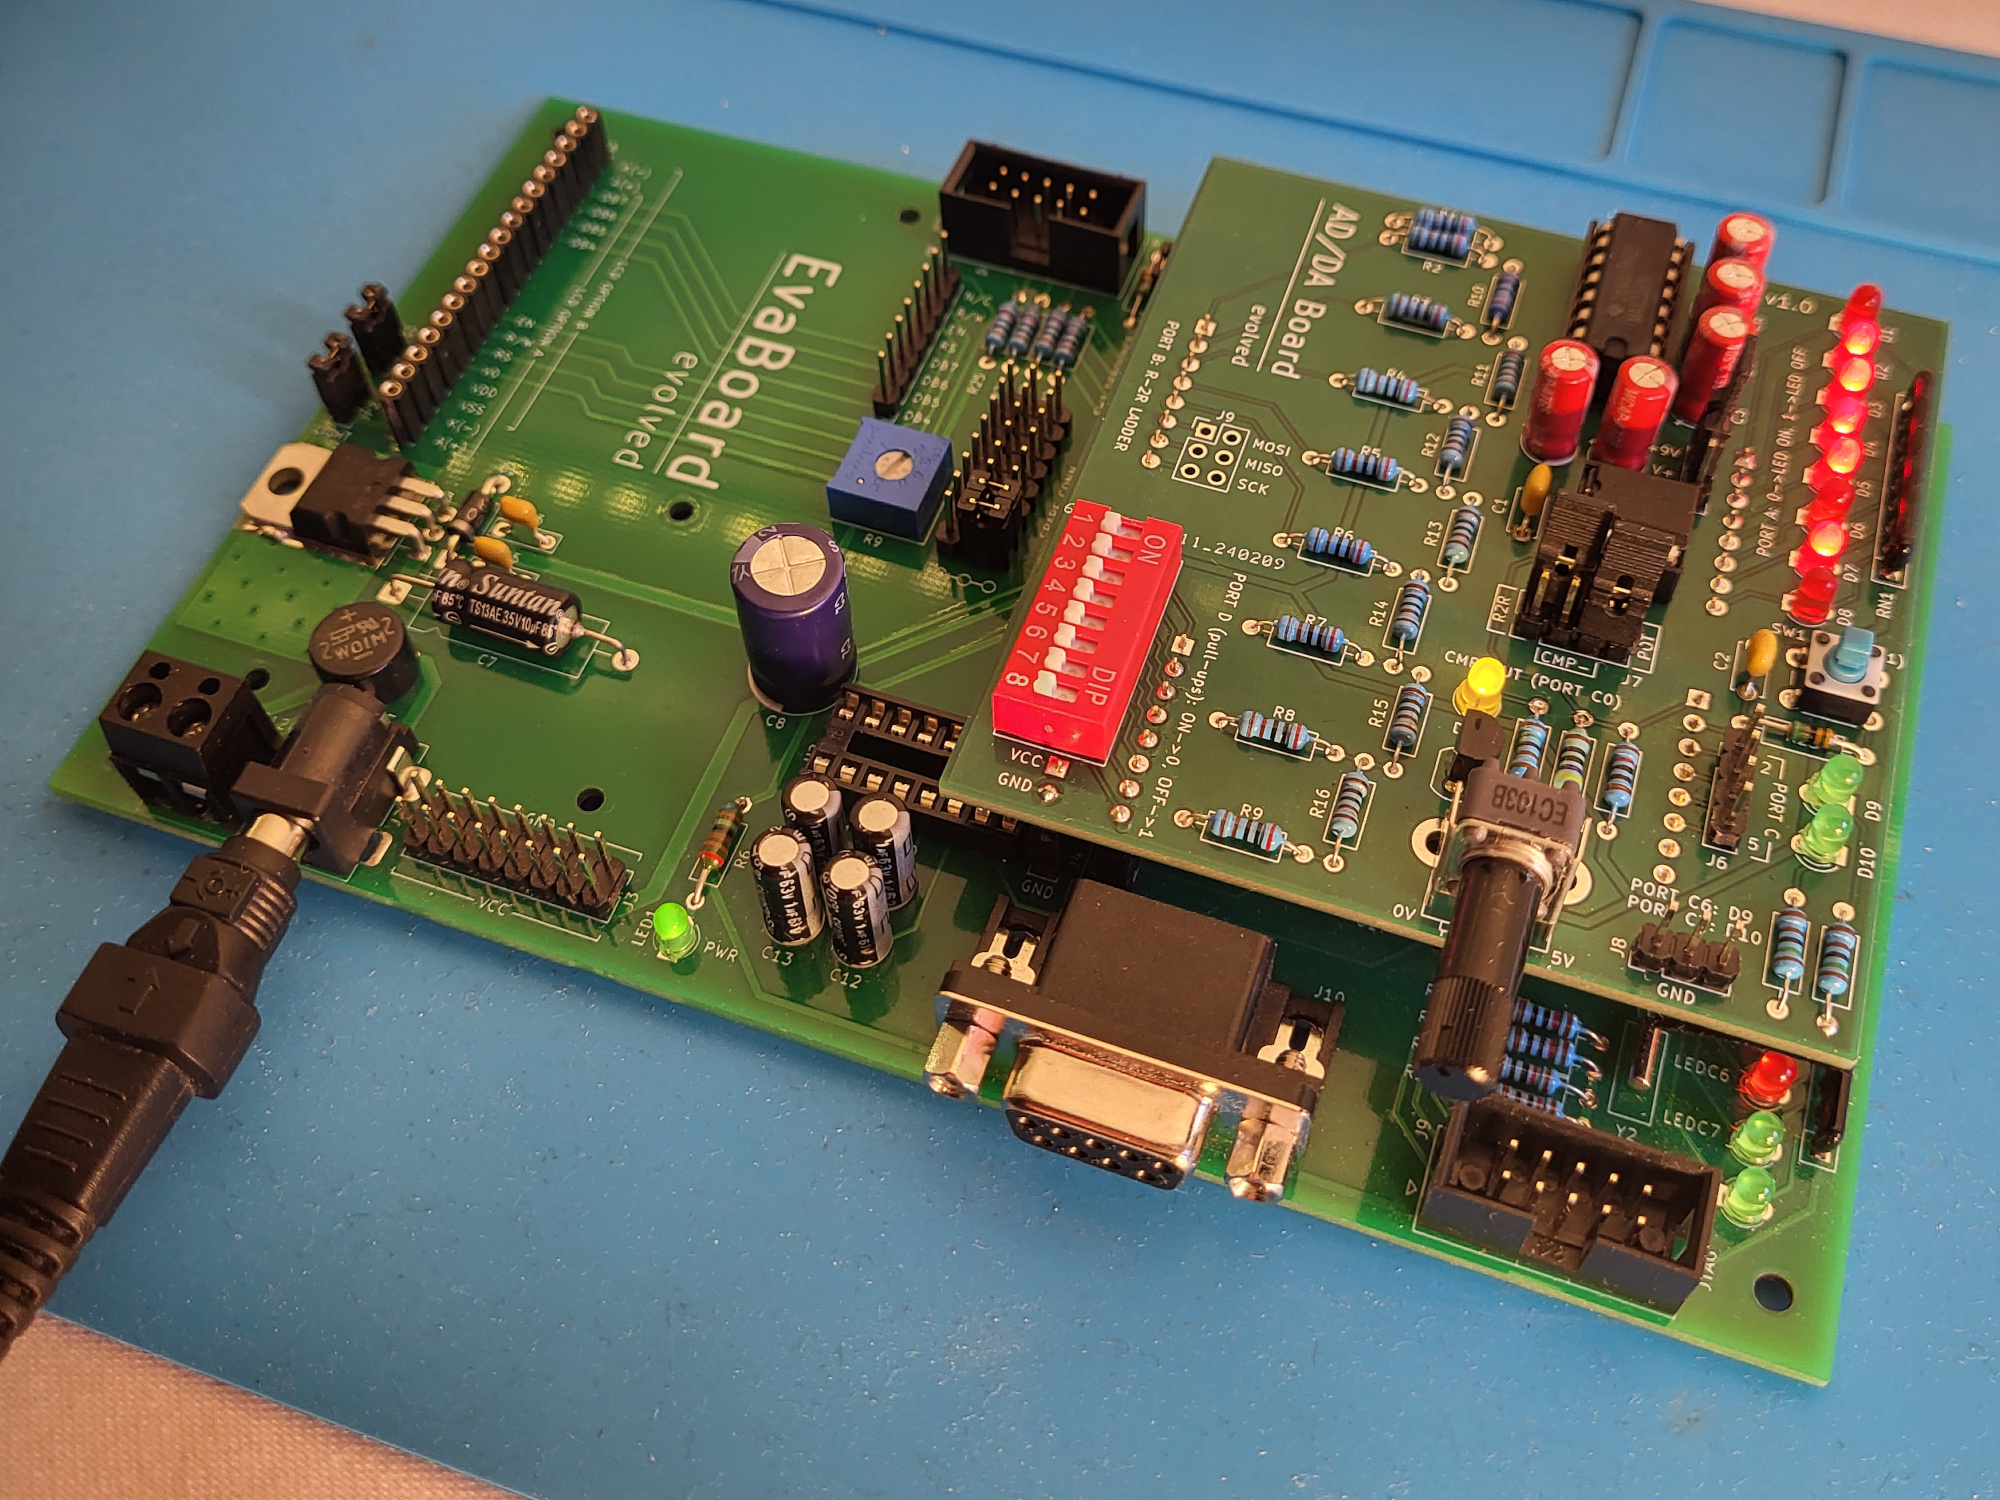
\includegraphics[width=.85\textwidth]{Pictures/ADC.jpg}
\caption{Setup for a Simple AD Converter (Using MAX232 for Supplying the Comparator)}
\label{fig:adc}
\end{figure}

\paragraph{Expected Result}
Select a voltage with the potentionmeter. Press the RESET button or disconnect and re-connect the power or reset the microcontroller via the programmer. 

The LEDs should show an increasing binary value which stops when the corresponding voltage from the R-2R ladder exceeds the potentiometer voltage. This is indicated by the ``CMP OUT'' LED lighting up. 

\begin{note}
This is a very primitive and slow ADC. You might view it as a linear search for the value where the comparator first outputs 1. You can improve it massively by using a more sophisticated search algorithm. 
\end{note}

\section{Known Issues}
In theory, the LEDs 1..10 and SW1 are superfluous. One could save on parts and use the LEDs and buttons on the evaluation board instead. However, this would require the PCB to be non-rectangular, probably offsetting any savings. 

\section{Version History}
\begin{description}
\item[v1.0] Initial release
\end{description}

\end{document}
